\documentclass[11pt]{article}

\usepackage{amsmath}
\usepackage{amssymb}
\usepackage{color}
\usepackage{cancel}
\usepackage{listings}
\usepackage{graphicx}

\textwidth=6.5in
\textheight=9in
\topmargin=-0.8in
\headheight=15.75pt
\headsep=.35in
\oddsidemargin=0.0in
\evensidemargin=0.0in

\newcommand{\Complex}{\mathbb{C}}
\newcommand{\Real}{\mathbb{R}}
\newcommand{\Dpt}{D_{+t}}
\newcommand{\Dmt}{D_{-t}}
\newcommand{\Dzt}{D_{0t}}
\newcommand{\Dpx}{D_{+x}}
\newcommand{\Dmx}{D_{-x}}
\newcommand{\Dzx}{D_{0x}}
\newcommand{\Oc}{\mathcal{O}}
\newcommand{\dx}{\Delta x}
\newcommand{\dt}{\Delta t}
\newcommand{\vnj}{v^{n}_j}
\newcommand{\vnpj}{v^{n+1}_j}
\newcommand{\vnjp}{v^{n}_{j+1}}
\newcommand{\vnjm}{v^{n}_{j-1}}
\newcommand{\vnpjp}{v^{n+1}_{j+1}}
\newcommand{\vnpjm}{v^{n+1}_{j-1}}
\newcommand{\vnpz}{v^{n+1}_{0}}
\newcommand{\vnz}{v^{n}_{0}}
\newcommand{\vnzm}{v^{n}_{-1}}
\newcommand{\vnpzm}{v^{n+1}_{-1}}
\newcommand{\vnNp}{v^{n}_{N+1}}
\newcommand{\vnpNp}{v^{n+1}_{N+1}}
\newcommand{\texp}[3]{\left[#1\right]^{#2}_{#3}}
\newcommand{\ux}{u_x}
\newcommand{\uxx}{u_{xx}}
\newcommand{\uxxx}{u_{xxx}}
\newcommand{\uxxxx}{u_{xxxx}}
\newcommand{\ut}{u_t}
\newcommand{\enj}{e^{n}_{j}}
\newcommand{\enpj}{e^{n+1}_{j}}
\newcommand{\enjp}{e^{n}_{j+1}}
\newcommand{\enjm}{e^{n}_{j-1}}
\newcommand{\unj}{u^{n}_{j}}
\newcommand{\unpj}{u^{n+1}_{j}}
\newcommand{\unjp}{u^{n}_{j+1}}
\newcommand{\unjm}{u^{n}_{j-1}}
\newcommand{\modu}[1]{\left | {#1} \right |}
\newcommand{\hVnp}{\hat{V}^{n+1}}
\newcommand{\hVn}{\hat{V}^n}
\newcommand{\bra}[1]{\left(#1\right)}

\begin{document}
\begin{flushright}
\small{MATH-6840\\
Vignesh Ramakrishnan\\
{\bf Due: Tuesday February 22, 2022}}
\end{flushright}

\begin{center}
\large{Problem Set 5}\\
\end{center}

\begin{enumerate}
  %%%%%
  %%%%%
  %%%%%
  \item (15 pts.) {\color{red}Consider the IBVP}
    \begin{align*}
      u_t & = \nu u_{xx}, \qquad x\in(0,1), \qquad 0 < t \le T_f\\
      u(x,0) & = f(x), \qquad x\in(0,1)\\
      u_x(0,t) & = \alpha(t), \qquad u(1,t) = \beta(t), \qquad t\ge 0.
    \end{align*}
    {\color{red}Using the grid }$x_j=j\dx$, $j=-1,0,\ldots,N+1$, $\dx=1/N${\color{red}, apply the following discretization}
    \begin{align*}
      \Dpt v_j^n & = \nu\Dpx\Dmx \left(\theta v_j^{n+1}+(1-\theta)v_j^{n}\right), && \qquad \hbox{for $j=0,1,\ldots,N$, $n=1,2,\ldots$}\\
      v_j^0 & = f(x_j) && \qquad \hbox{for $j=0,1,\ldots,N $}\\
      \Dzx v_0^n & = \alpha(t_n) && \qquad \hbox{for $n=0,1,\ldots$}\\
      \nu\Dpx\Dmx v_N^n & = \beta^{'}(t_n) && \qquad \hbox{for $n=0,1,\ldots$},
    \end{align*}
    {\color{red}where} $\theta\in[0,1]${\color{red} is a parameter (note }$\theta=1${\color{red} corresponds to backward Euler, }$\theta=\frac{1}{2}${\color{red} corresponds to the trapezoidal rule, and $\theta=0$ corresponds to forward Euler. }
    
    \begin{enumerate}
      \item {\color{blue}Determine the order-of-accuracy (consistency) of the scheme including both the interior 	discretization and the boundary conditions. }
      A Taylor's series expansion of the exact solution using the given discretization will help in determining the order of accuracy of this scheme given to us. 
      \begin{align*}
      \Dpt \unj = & \  \frac{\unpj - \unj}{\dt} \\
      \unpj - \unj =& \ \texp{\cancel{u} + \dt \ \ut + \frac{\dt^2}{2!} \ u_{tt}}{n}{j} - \cancel{\unj} \\
      \Dpt \unj = & \ \texp{\ut + \frac{\dt}{2!} \ u_{tt} + \Oc(\dt^2) }{n}{j} 
      \end{align*}
      
      \begin{align*}
      \nu \ \Dpx\Dmx \ \left(\theta \unpj + (1-\theta)\unj \ \right) = & \ \nu \theta \Dpx\Dmx \texp{u + \dt \ \ut + \Oc(\dt^2)}{n}{j} + \nu (1-\theta)\Dpx\Dmx \unj \\
      = & \ \cancel{\nu \theta \ \Dpx\Dmx \unj} + \nu\theta \Dpx\Dmx \texp{\dt \ut + \Oc(\dt^2)}{n}{j} \\
      & \ + \nu\Dpx\Dmx\unj -\cancel{\nu\theta\Dpx\Dmx \unj}   \\
      = & \  \nu\theta \Dpx\Dmx \texp{\dt \ut + \Oc(\dt^2)}{n}{j} + \nu\Dpx\Dmx\unj
      \end{align*}
      
      Here,
      \begin{align*}
      \nu\Dpx\Dmx\unj = & \ \nu \ \texp{\uxx + \Oc(\dx^2)}{n}{j} \\
      \nu\theta\Dpx\Dmx\texp{ \dt \ \ut + \Oc(\dt^2)}{n}{j} = & \ \nu \theta \ \dt \Dpx\Dmx \texp{\ut}{n}{j} + \Oc(\dt^2) \\
      = & \ \nu\theta \ \dt \frac{\left([\ut]^n_{j+1} -2[\ut]^n_j + [\ut]^n_{j-1}\right)}{\dx^2} \\
      = & \ \nu\theta \ \dt \texp{u_{xxt} + \frac{2\dx^2}{4!}u_{xxxxt} + \Oc(\dx^4)}{n}{j} \\
      = & \ \nu\theta \ \dt \texp{u_{xxt} + \Oc(\dx^2)}{n}{j}\\
      \end{align*}
      
      Substituting them in the above equation results in,
      \begin{align*}
       \nu \ \Dpx\Dmx \ \left(\theta \unpj + (1-\theta)\unj \ \right) = & \ \nu \ \texp{\uxx + \Oc(\dx^2)}{n}{j} + \nu\theta \ \dt \texp{u_{xxt} + \Oc(\dx^2)}{n}{j} \\
       \tau^{n}_{j} =  \ \texp{\ut + \frac{\dt}{2!} \ u_{tt} + \Oc(\dt^2) }{n}{j}  & - \nu \ \texp{\uxx + \Oc(\dx^2)}{n}{j} + \nu\theta \ \dt \texp{u_{xxt} + \Oc(\dx^2)}{n}{j} \\
      \end{align*}
      \begin{align*}
             \tau^{n}_{j} = &  \ {\color{red}\cancel{\ut}} + \dt \left(\frac{1}{2}u_{tt} - \nu\theta u_{xxt}\right) + \Oc(\dt^2) -  \ {\color{red}\cancel{\nu \ \uxx}} + \Oc(\dx^2) \\
             \tau^{n}_{j} = & \ \dt u_{tt}\left(\frac{1}{2} - \theta \right) + \Oc(\dt^2) + \Oc(\dx^2)
      \end{align*}
      If $\theta = \frac{1}{2}$, this scheme is second order accurate in both time and space, but if it isn't, then it is first order accurate in time and second order accurate in space.\\
      %%%
      %%%
      %%%
      \item {\color{blue}Using normal mode stability theory, determine the stability of the scheme taking account of the boundary conditions. Please use the notation that} $r=\frac{\nu\dt}{\dx^2}$. {\color{blue} Hint: for stability you need only consider the error equation so that the boundary conditions can be taken as homogeneous.}\\
      
      Expanding this discretization, we get,
      \begin{align*}
      -r\theta \ \vnpjp + \left(1+2r\theta\right)\vnpj - r\theta \ \vnpjm = & \ r\left(1-\theta \right)\vnjp + \left(1-2r\left(1-\theta \right)\right)\vnj + r\left(1-\theta\right)\vnjm
      \end{align*}
      Let $\vnj = ca^n k^j$, 
      \begin{align*}
      -r\theta \bra{ak}\cancel{\vnj} + \bra{1-2r\theta}a\cancel{\vnj} -r\theta \bra{\frac{a}{k}}\cancel{\vnj} = & \ r\bra{1-\theta} k\cancel{\vnj} + \bra{1-2r\bra{1-\theta}}\cancel{\vnj} + r\bra{1-\theta}\frac{1}{k} \cancel{\vnj} \\
      -r\theta a\bra{k + \frac{1}{k}} + \bra{1-2r\theta}a = &\ r\bra{1-\theta}\bra{k + \frac{1}{k}} + \bra{1-2r\bra{1-\theta}}\\
      \bra{a-2ra\theta} - \bra{1-2r\bra{1-\theta}} = & \ \bra{k + \frac{1}{k}}\bra{r\bra{1-\theta} + ra\theta} \\
      \bra{k+\frac{1}{k}} = & \ \frac{\bra{a-1}\bra{1-2r}-2r\theta}{r+r\theta\bra{a-1}} = \mu \\
      \end{align*}
      \begin{align*}
      \frac{k^2 + 1}{k} =& \ \mu \\
      k^2 -\mu k + 1 = & \ 0 \\
      \implies k = & \ \frac{\mu \pm \sqrt{\mu^2-4}}{2} = \frac{\mu}{2} \pm \sqrt{\bra{\frac{\mu}{2}}^2 - 1}
      \end{align*}
      Let $\frac{\mu}{2} = \cos\bra{\xi}$, 
      \begin{align*}
      k = & \ \cos\bra{\xi} \pm i \sin\bra{\xi} = e^{\pm \ i \xi}
      \end{align*}
      \begin{align*}
      \vnj = & \ c_1 e^{i\xi j} + c_2 e^{-i\xi j} \\
      v^{n}_{0} = & \ c_1 + c_2 = 0 \bra{\text{Assumption - Homogenous BC}} \\
      v^{n}_{N}= & \ c_1\bra{e^{i\xi N} - e^{-i\xi N}} = i \ 2c_1 \sin\bra{N \xi} = 0 \\
      \end{align*}
      \begin{align*}
      \implies N\xi = & \ p\pi \\
      \xi = & \ \frac{p\pi}{N}  \\
      \mu = & \ 2\cos\bra{\frac{p\pi}{N}} = \frac{\bra{a-1}\bra{1-2r}-2r\theta}{r+r\theta\bra{a-1}} \\
      \text{Let, }\cos\bra{\frac{p\pi}{N}} =& \delta \\
      \implies 2\delta\bra{r+r\theta\bra{a-1}} = & \ \bra{a-1}\bra{1-2r} -2r\theta \\
      2r\delta + 2\delta r\theta \bra{a-1} = & \ \bra{a-1}\bra{1-2r} -2r\theta \\
      2r\delta + 2r\theta = & \ \bra{a-1}\bra{1-2r - 2\delta r\theta} \\
      a = & \ 1 + \frac{2r\delta + 2r\theta}{1-2r-2r\delta \theta}
      \end{align*}
      If $\modu{a}\leq 1$, then,
      \[ 
      -1 \leq 1 + \frac{2r\delta + 2r\theta}{1-2r-2r\delta \theta} \leq 1
      \]
      From the right hand side inequality, 
      \begin{align*}
      2r\delta +2r\theta \leq 1 - 2r - 2r\delta \theta \\
      2r\bra{\delta + \theta} \leq 1- 2r\bra{1+\delta \theta} \\
      2r\bra{1+\delta + \theta + \delta \theta} \leq 1 \\
      r \leq \frac{1}{2\bra{1+\delta + \theta + \delta \theta}}
      \end{align*}
      This makes sense because when $\delta=0, \theta = 0$, $r$ becomes what we already know, $\leq \frac{1}{2}$. \\
      %%%
      %%%
      %%%
      \item {\color{blue}Based on the above, how do you expect the scheme converge with respect to grid parameters? Why?} \\
      
      The scheme will converge well as long as, 
      \[
      \dt \leq \frac{\dx^2}{2\nu\bra{1+\delta + \theta + \delta \theta}}
      \]
    \end{enumerate}

  %%%%%
  %%%%%
  %%%%%
  \item  (20 pts.){\color{red} Here you will take steps to implement the discretization described in \#1.}
    \begin{enumerate}
      \item {\color{blue}Carefully write down the} $N+3$ {\color{blue}linear equations that must be solved at each time step. Present this linear system.}
        \begin{align*}
      -r\theta \ \vnpjp + \left(1+2r\theta\right)\vnpj - r\theta \ \vnpjm = & \ r\left(1-\theta \right)\vnjp + \left(1-2r\left(1-\theta \right)\right)\vnj + r\left(1-\theta\right)\vnjm
      \end{align*}
      \begin{align*}
       \Dzx v_0^n & = \alpha(t_n) && \qquad \hbox{for $n=0,1,\ldots$}\\
       \Dzx v_0^{n+1} & = \alpha(t_{n+1}) && \qquad \hbox{for $n=0,1,\ldots$}\\
      \nu\Dpx\Dmx v_N^n & = \beta^{'}(t_n) && \qquad \hbox{for $n=0,1,\ldots$},\\
      \nu\Dpx\Dmx v_N^{n+1} & = \beta^{'}(t_{n+1}) && \qquad \hbox{for $n=0,1,\ldots$},
      \end{align*}
      \begin{align*}
      - v^{n+1}_{-1} + v^{n+1}_{1} =& \ 2\dx \alpha(\bra{n+1}\dt) \\
      v^{n+1}_{N-1} -2v^{n+1}_N + v^{n+1}_{N+1} = & \ \frac{\dx^2}{\nu} \beta^{'}(\bra{n+1}\dt)
      \end{align*}
      \begin{align*}
      \begin{bmatrix}
      -1 & 0 &  1& \ldots & \ldots & \ldots &  \ldots & \dots\\
      -r\theta & \bra{1+2r\theta} & -r\theta & \ldots & \ldots & \ldots & \ldots & \dots\\
      0 & -r\theta & \bra{1+2r\theta} & -r\theta & \ldots & \ldots &  \ldots & \dots \\
      \vdots & \vdots & \vdots & \vdots & \vdots & \vdots & \vdots & \vdots \\
      \vdots & \vdots & \vdots & \vdots & \vdots & \vdots  & \vdots & \vdots\\
      \vdots & \vdots & \vdots & \vdots & \vdots & \vdots & \vdots & \vdots \\
      0 & 0 & 0 & 0 & 0 & -r\theta & \bra{1+2r\theta} & -r\theta \\
      0 & 0 & 0 & 0 & 0 & 1 & -2 & 1 \\
      \end{bmatrix} 
      \begin{bmatrix}
      v^{n+1}_{-1}\\
      v^{n+1}_{0} \\
      v^{n+1}_{1} \\
      \vdots \\
      \vdots \\
      \vdots \\
      v^{n+1}_{N} \\
      v^{n+1}_{N+1}
      \end{bmatrix} = \\
      \begin{bmatrix}
      2\dx \ \alpha\bra{\bra{n+1}\dt} \\
      r\bra{1-\theta}v^{n}_{1} + \bra{1-2r\bra{1-\theta}}v^{n}_{0} + r\bra{1-\theta}v^{n}_{-1} \\
      r\bra{1-\theta}v^{n}_{2} + \bra{1-2r\bra{1-\theta}}v^{n}_{1} + r\bra{1-\theta}v^{n}_{0} \\
      \vdots \\
      \vdots \\
      \vdots \\
      r\bra{1-\theta}v^{n}_{N-1} + \bra{1-2r\bra{1-\theta}}v^{n}_{N} + r\bra{1-\theta}v^{n}_{N+1} \\
      \frac{\dx^2}{\nu}\beta^{'}\bra{\bra{n+1}\dt}
      \end{bmatrix}
      \end{align*}
      There are $N+1$ equations for solution variables $v^{n+1}_{0}$ to $v^{n+1}_{N}$. Since there are two ghost nodes added, two extra equations are added at the top and at the bottom row of the linear system of equations and this constitutes to a total of $N+3$ equations. \\
      %%%
      %%%
      %%%
      \item {\color{blue}Now implement the scheme in code using the solution} $u_{ex} = e^{-\nu k^2 t} \sin(kx)${\color{blue}, from which you must determine }$f(x)${\color{blue},} $\alpha(t)${\color{blue}, and }$\beta(t)${\color{blue}. Note that much of the infrastructure can be adopted from the solution to PS \#3 problem \#4.} \\
      
      Through method of manufactured solutions, if $u_{ex} = e^{-\nu k^2 t}\sin\bra{kx}$, then 
      \begin{align*}
      u\bra{x,t=0} = & \ \sin\bra{kx} = f\bra{x} \\
      u_{x}\bra{x=0,t} = & \ ke^{-\nu k^2 t} \cos \bra{0} = k e^{-\nu k^2 t } = \alpha \bra{t} \\
      u\bra{x=1,t} = & \ e^{-\nu k^2 t} \sin\bra{k} = \beta\bra{t} \\
      u_t \bra{x=1,t} = & \ -\nu k^2 \sin\bra{k} e^{-\nu k^2 t} =   \beta^{'}\bra{t}
      \end{align*}
      
      The code written for this question is included below. 
      \lstinputlisting[language=Matlab, numbers=left, stepnumber=1, firstline=1,caption={Heat Equation - weighted Implicit scheme},label=code:myCode,frame=single]{HeatEqn_ImplicitForcing.m}
      
      %%%
      %%%
      %%%
      \item {\color{blue}Taking} $\nu=1$, $k=2$ {\color{blue}and} $T_f=.4${\color{blue}, perform a convergence study with }$N=20, 40, 80, 160$ {\color{blue} using} $\theta=1$ {\color{blue} and }$r=\frac{\nu\dt}{\dx}\approx 0.9$ {\color{blue} (as usual, the time step may be slightly modified so the simulation actually attains the final time). Present plots of the solution and plots of the error at the final time for each grid resolution. Also present a log-log plot of the maximum error vs. the grid size, as well as a reference line indicating the expected convergence rate.}
      %%%
      %%%
      %%%
      \item {\color{blue}Taking} $\nu=1$, $k=2$ {\color{blue}and} $T_f=.4${\color{blue}, perform a convergence study with }$N=20, 40, 80, 160$ {\color{blue} using} $\theta=\frac{1}{2}$ {\color{blue} and }$r=\frac{\nu\dt}{\dx}\approx 0.9$ {\color{blue} (as usual, the time step may be slightly modified so the simulation actually attains the final time). Present plots of the solution and plots of the error at the final time for each grid resolution. Also present a log-log plot of the maximum error vs. the grid size, as well as a reference line indicating the expected convergence rate.} \\
      
      Combining both part (c) and part (d), the results are presented below in Fig~\ref{fig:q21}, Fig~\ref{fig:q22}, Fig~\ref{fig:q23} \\
    \begin{figure}[htp]
    \begin{tabular}{|c|c|}
    \hline
    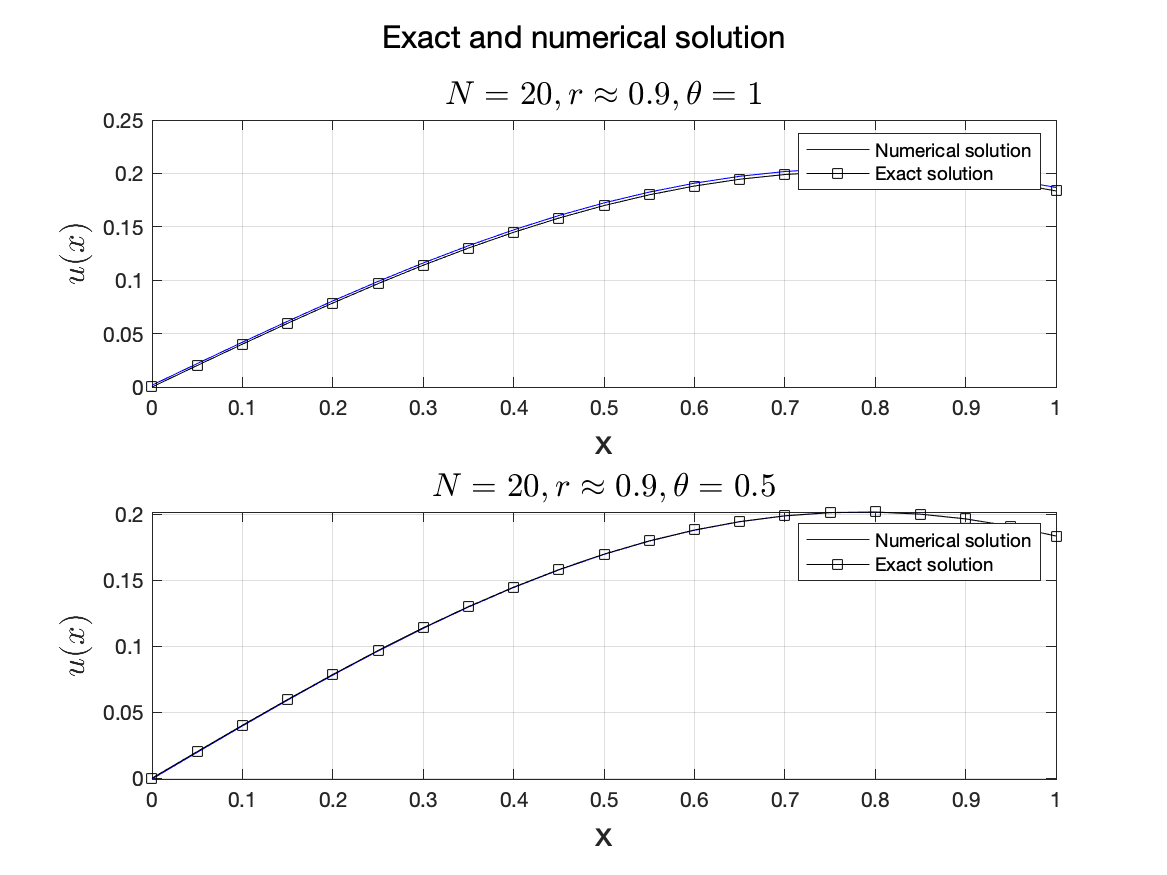
\includegraphics[width=3.5in]{solN1} & 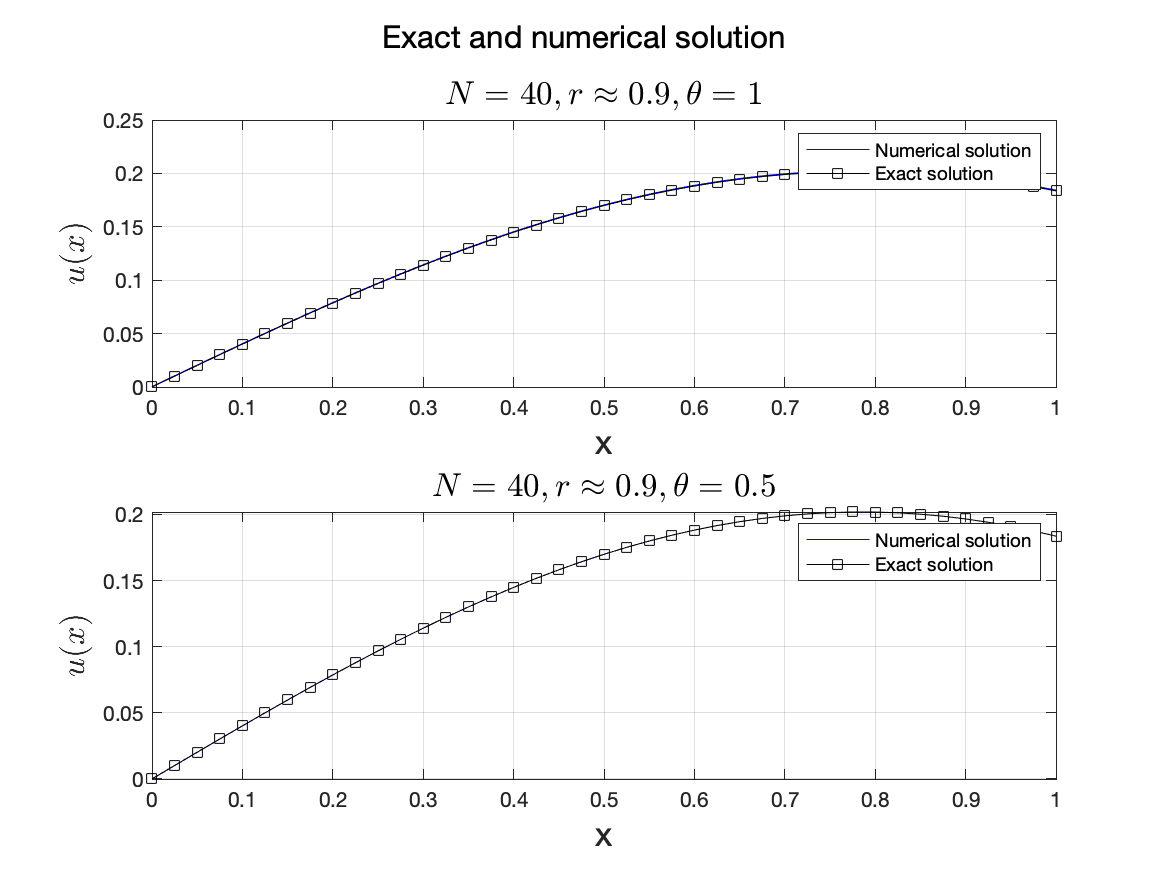
\includegraphics[width=3.5in]{solN2} \\
    \hline
    \end{tabular}
    \begin{tabular}{|c|c|}
    \hline
    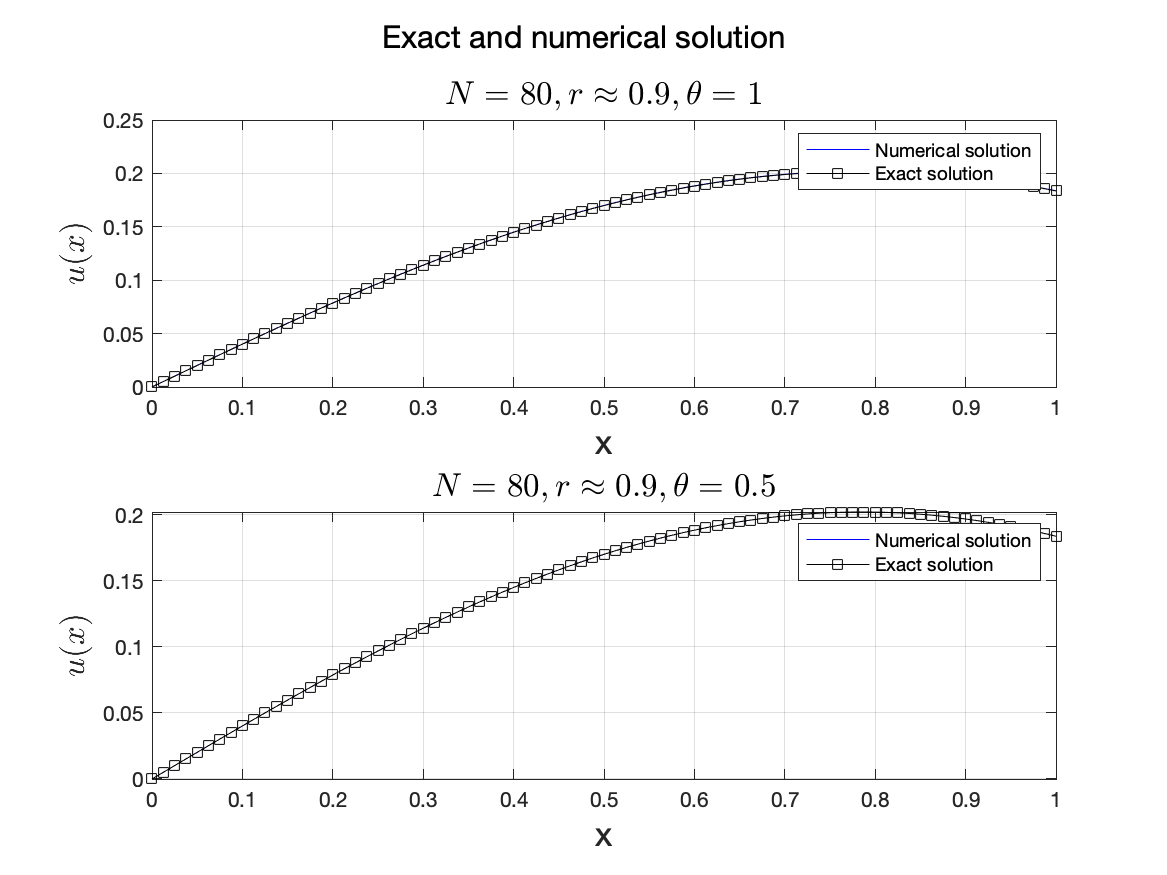
\includegraphics[width=3.5in]{solN3} & 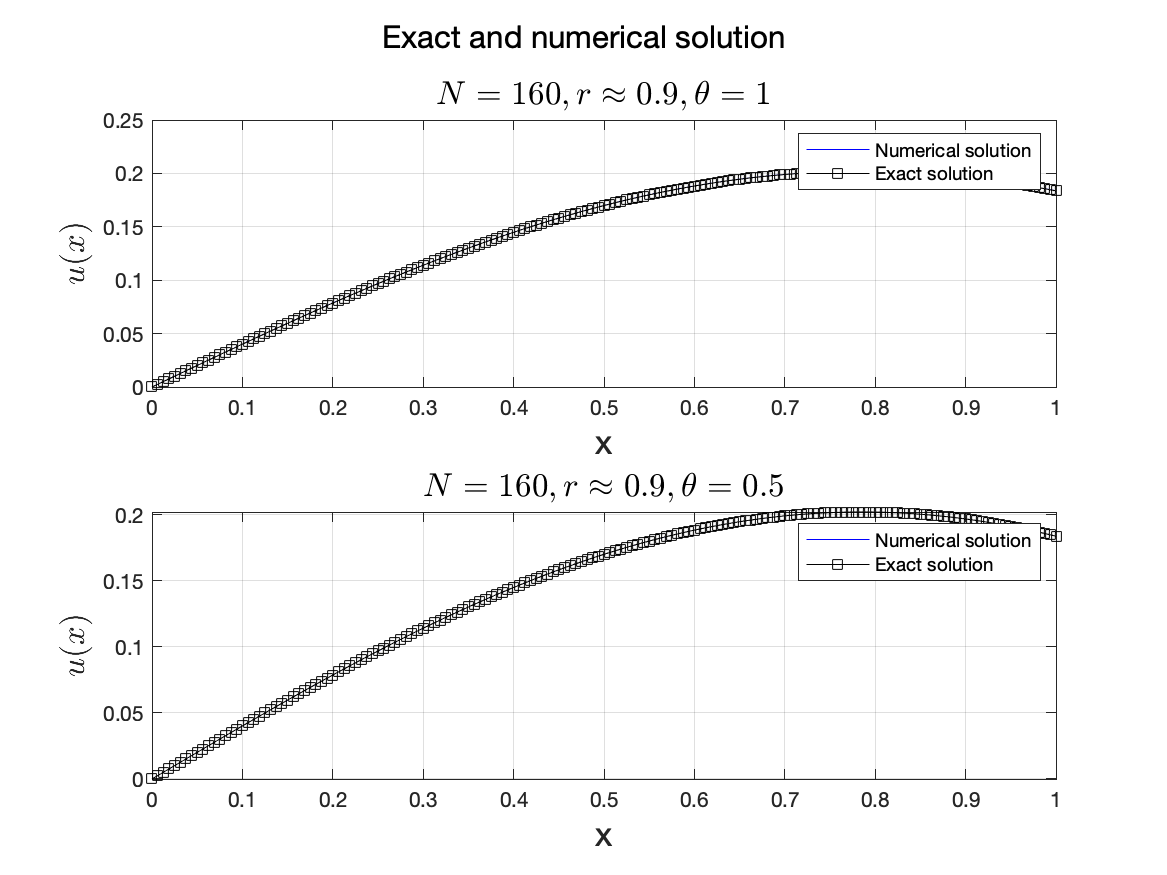
\includegraphics[width=3.5in]{solN4}\\
    \hline
    \end{tabular}
    \caption{Solution plots}
    \label{fig:q21}
    \end{figure}
    
    \begin{figure}[htp]
    \begin{tabular}{|c|c|}
    \hline
    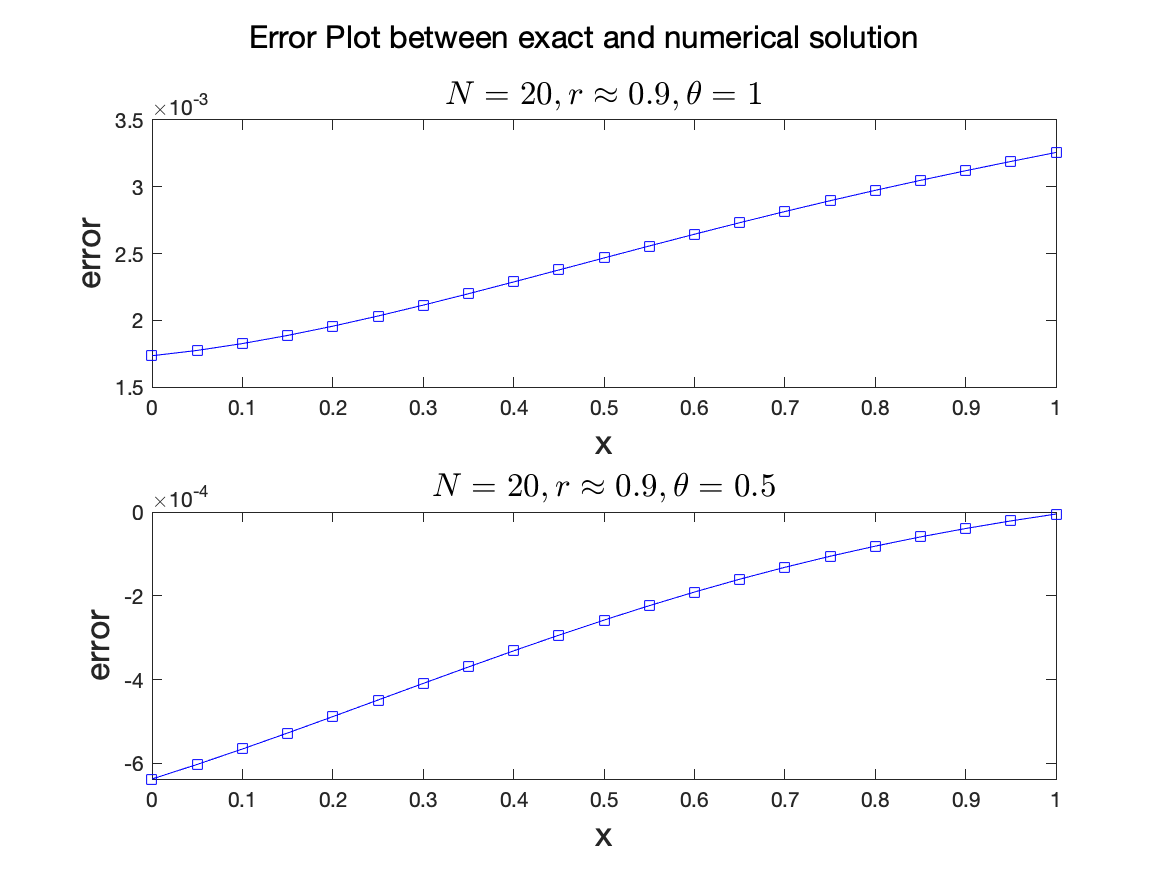
\includegraphics[width=3.5in]{N1} & 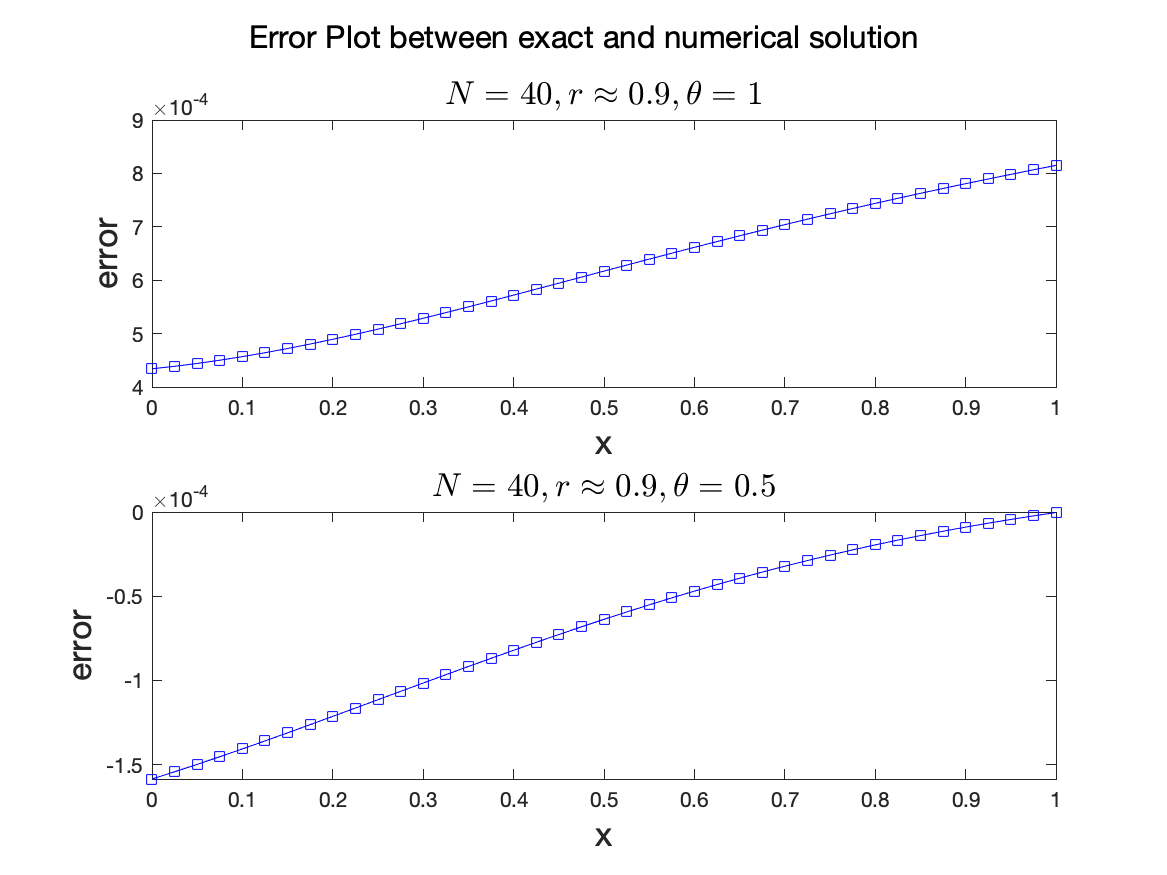
\includegraphics[width=3.5in]{N2} \\
    \hline
    \end{tabular}
    \begin{tabular}{|c|c|}
    \hline
    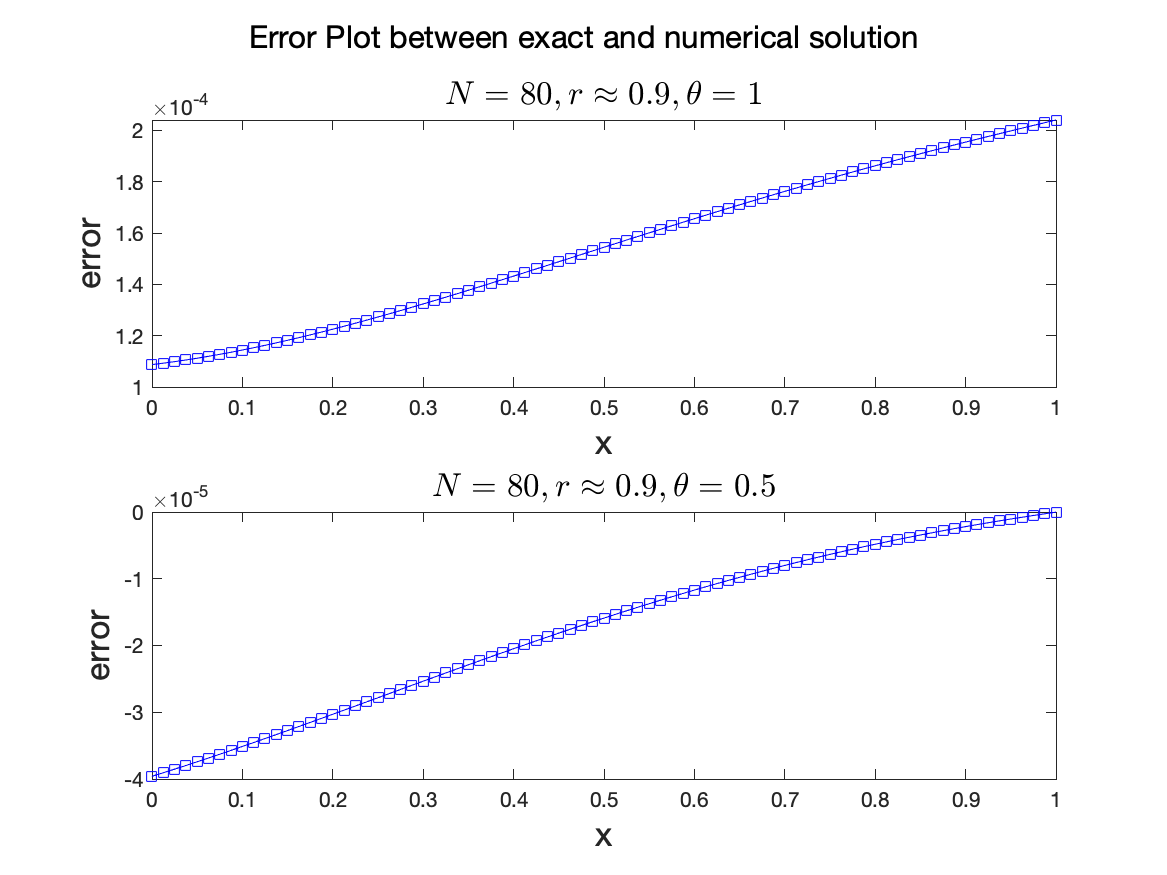
\includegraphics[width=3.5in]{N3} & 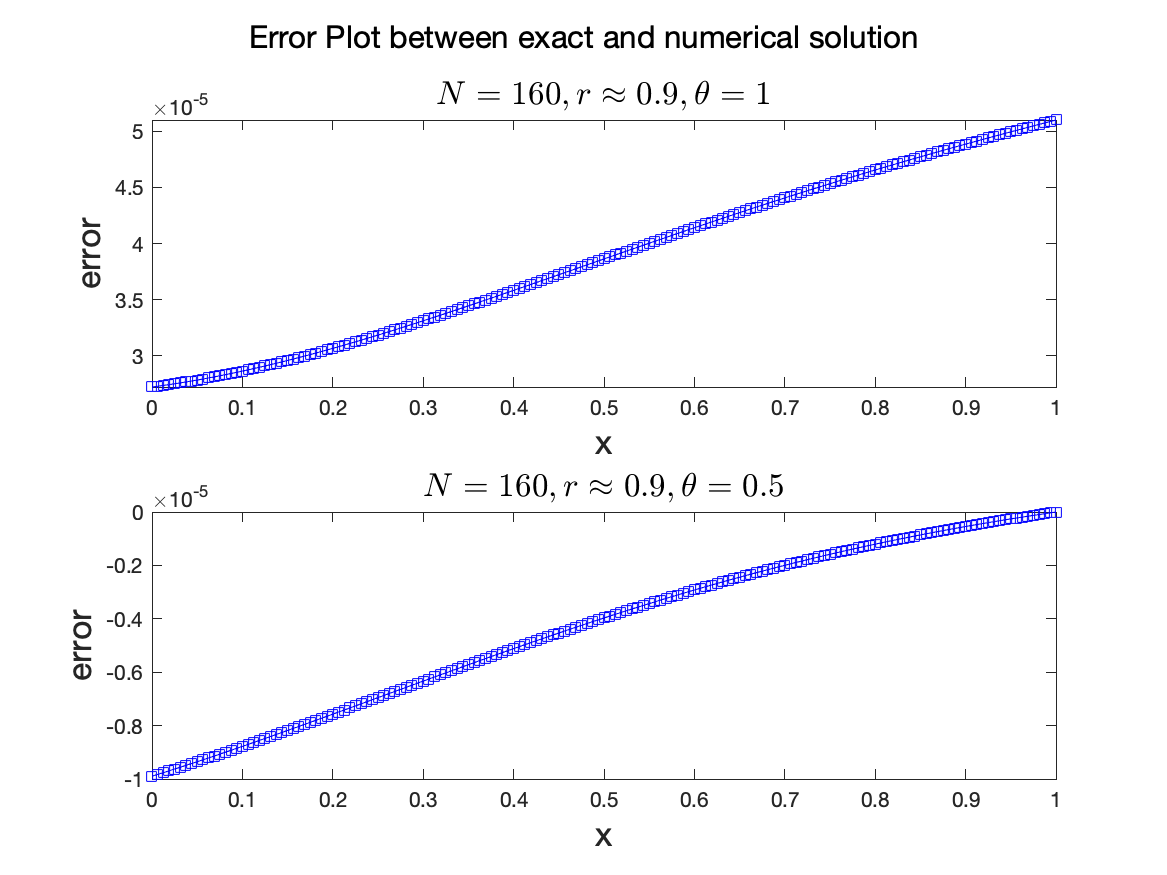
\includegraphics[width=3.5in]{N4}\\
    \hline
    \end{tabular}
    \caption{Error plots at different resolutions}
    \label{fig:q22}
    \end{figure}
    \begin{figure}[htp]
    \centering
    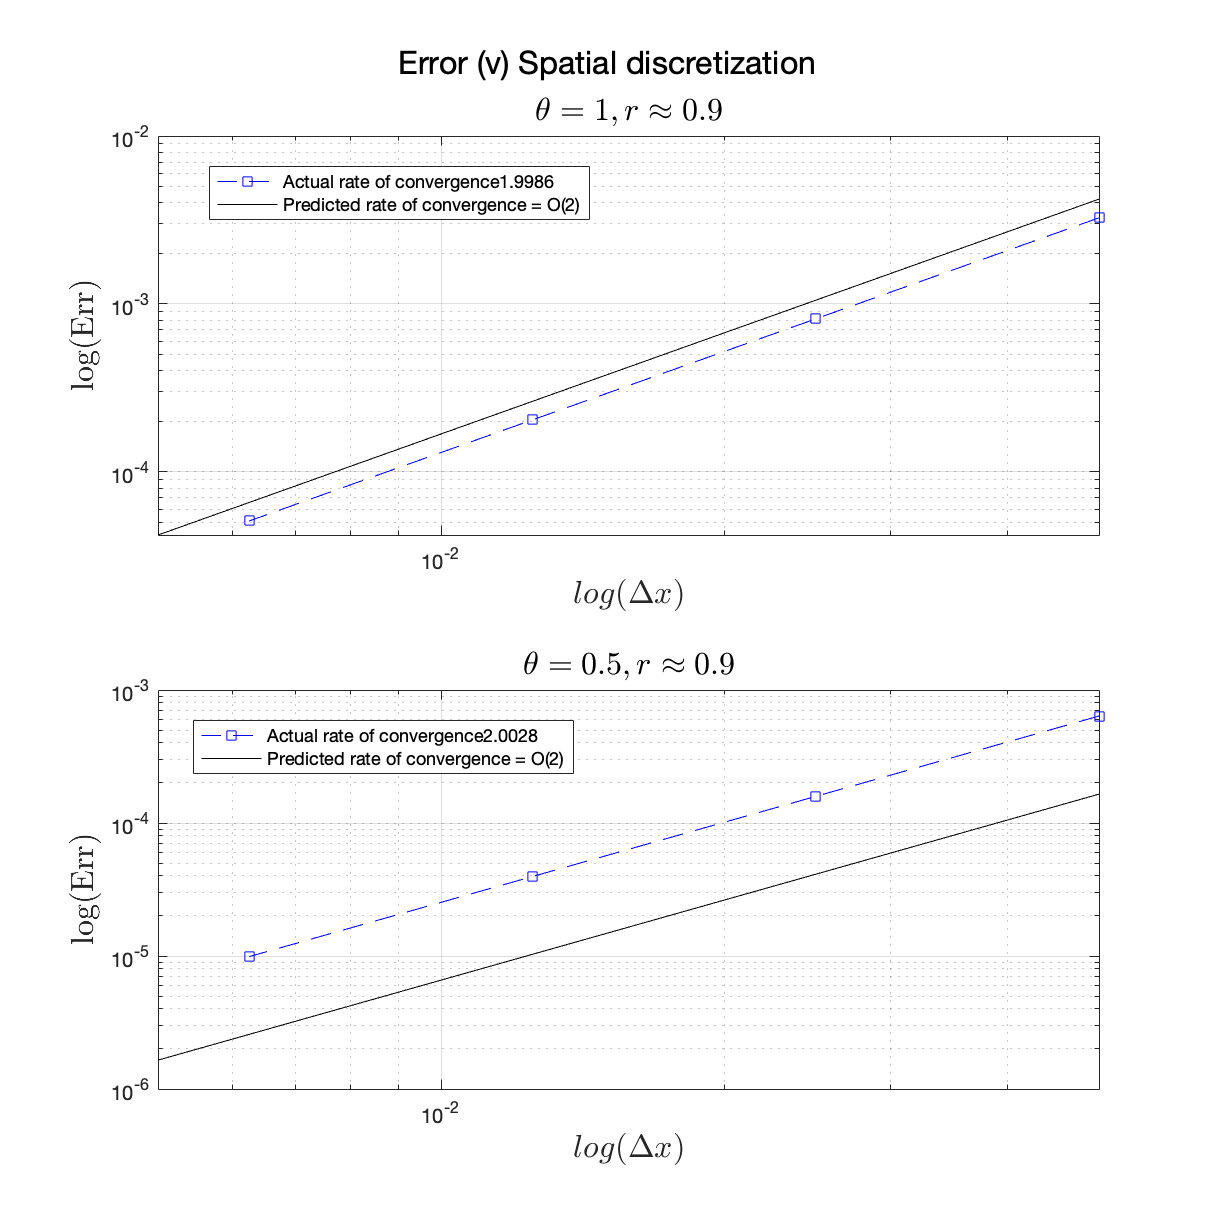
\includegraphics[width=5in]{ErrPlot}
    \caption{Log-Log plot of the infinity norm of error and spatial discretization}
    \label{fig:q23}
    \end{figure}
    \end{enumerate}
  %%%%%
  %%%%%
  %%%%%
  \item (10 pts.) {\color{red}In HW \#2 problem \#2, we investigated the leapfrog scheme with a centered spatial discretization for the heat equation and experienced some difficulty in computing solutions.}
    \begin{enumerate}
      \item {\color{blue}Determine the amplification factor of the discrete operator, and make surface plots of the amplitude of the amplification factor as a function of discrete wave number and the parameter} $r=\frac{\nu\dt}{\dx^2}${\color{blue}. Note there are two roots and you should produce one plot for each root.} \\
      
      The Leapfrog scheme is written as,
      \begin{align*}
      \Dzt\vnj = & \ \nu \ \Dpx\Dmx \vnj \\
      \vnpj  =& \  v^{n-1}_{j} + 2r\bra{\vnjp-2\vnj+\vnjm}
      \end{align*}
      Let $\vnj = ca^{n}k^{j}$, then the equation reduces to
      \begin{align*}
      a = & \ \frac{1}{a} + 2r\bra{k-2+\frac{1}{k}} \\
      \bra{a-\frac{1}{a}} = & \ 2r\bra{k + \frac{1}{k}}-4r
      \end{align*}
      \begin{align*}
      \mu &= \bra{\frac{a^2-1}{2ar}+2} = \bra{k+\frac{1}{k}}
      \end{align*}
      \begin{align*}
      k = & \ \frac{-\mu \pm \sqrt{\mu^2-4}}{2} = \frac{\mu}{2} \pm \sqrt{\bra{\frac{\mu}{2}}^2-1}
      \end{align*}
      If $\cos\xi = \frac{\mu}{2}$, then,
      \begin{align*}
      k = & \ e^{\pm i \xi}
      \end{align*}
      Assuming Homogeneous Boundary conditions,
      \begin{align*}
      v^n_{0} = & \ c_1 + c_2 = 0 \\
      v^n_{N} = & \ c_1\bra{e^{i\xi N} - e^{-i\xi N}} = 0
      \end{align*}
      Solving for $\xi$ yields, $\xi = \frac{p\pi}{N}$
      \begin{align*}
      \frac{\mu}{2} = & \ \cos\bra{\frac{p\pi}{N}} = \delta 
      \end{align*}
      \[  a^2 + 4ar\bra{1-\delta} - 1 =   0 \]
      Solving for $a$ results in two solutions
      \begin{align*}
      a_1 = & \ \frac{-4r\bra{1-\delta} + \sqrt{16r^2\bra{1-\delta}^2 + 4}}{2} \\
      a_2 = & \ \frac{-4r\bra{1-\delta} - \sqrt{16r^2\bra{1-\delta}^2 + 4}}{2}
      \end{align*}
      The surface plots are shown below, in Fig~\ref{fig:q3}
      \begin{figure}[htp]
      \centering
      \begin{tabular}{|c|}
      \hline \\
      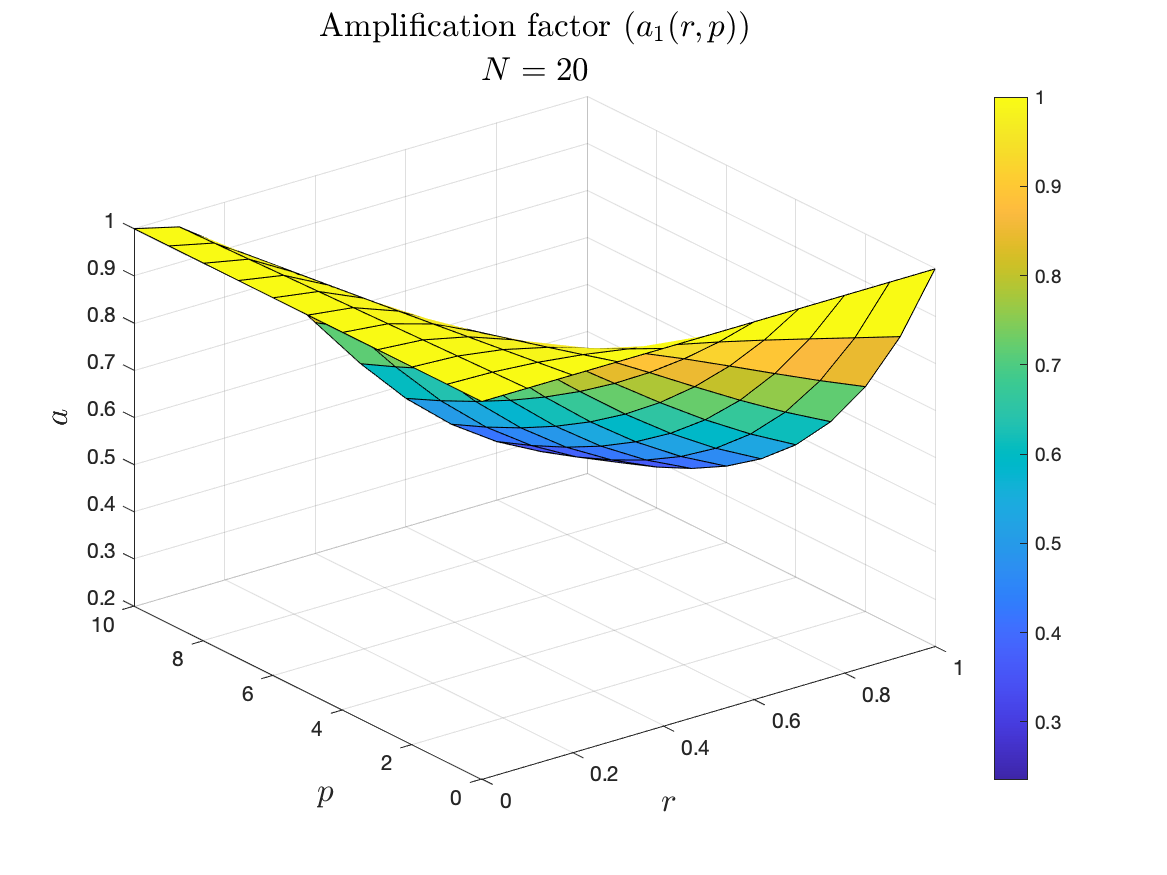
\includegraphics[width=4in]{a1} \\
      \hline \\
      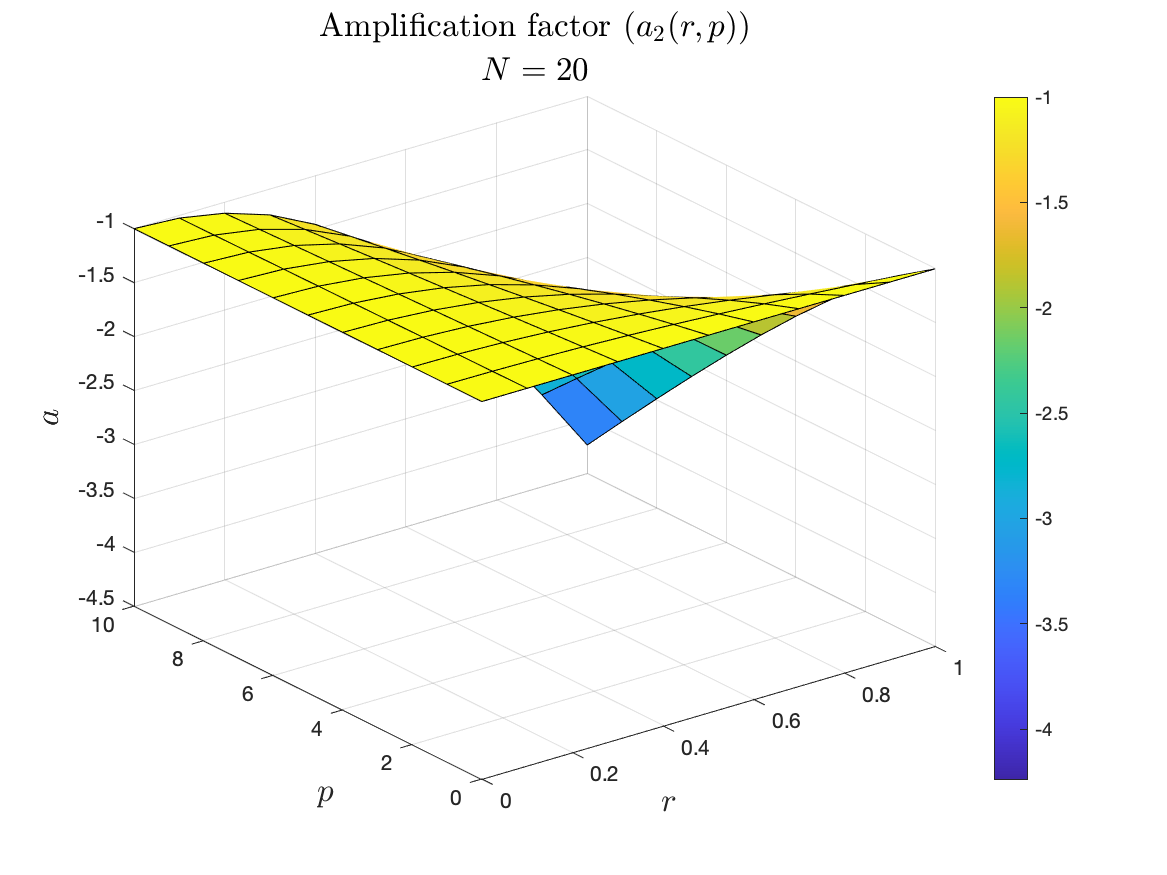
\includegraphics[width=4in]{a2} \\
      \hline
      \end{tabular}
      \caption{Amplification factor}
      \label{fig:q3}
      \end{figure}
      \item {\color{blue}Determine if the scheme is stable for any choice of the parameter }$r>0$ {\color{blue} (hint: you may find it useful to use the plots from (a) as a guide). How do these results help to explain the behavior that we experienced in HW \#2 problem \#2.} \\
      There is one root of the amplification factor $a$ where when, $r >$ somewhere around $0.5$, the magnitude of the amplification factor becomes $>1$ and hence the scheme becomes unstable. 
      
    \end{enumerate}

    
  \end{enumerate}
    
  
\end{document}
